
%(BEGIN_QUESTION)
% Copyright 2009, Tony R. Kuphaldt, released under the Creative Commons Attribution License (v 1.0)
% This means you may do almost anything with this work of mine, so long as you give me proper credit

Read and outline the ``Complementary Valve Sequencing'' subsection of the ``Split-Ranging'' section of the ``Control Valves'' chapter in your {\it Lessons In Industrial Instrumentation} textbook.  Note the page numbers where important illustrations, photographs, equations, tables, and other relevant details are found.  Prepare to thoughtfully discuss with your instructor and classmates the concepts and examples explored in this reading.

\underbar{file i04208}
%(END_QUESTION)





%(BEGIN_ANSWER)


%(END_ANSWER)





%(BEGIN_NOTES)

Complementary split-ranging is when two control valves operate off the same signal, with their positions being mathematical complements of each other (i.e. the sum of both valve stem positions always equals 100\%).  Useful for flow mixing and flow diverging applications.  Three-way mixing/diverting valves are a mechanical alternative to two complementary-ranged control valves.

\vskip 10pt

The following illustration graphically depicts this type of valve sequencing:

$$\includegraphics[width=15.5cm]{i04208x01.eps}$$





\vskip 20pt \vbox{\hrule \hbox{\strut \vrule{} {\bf Suggestions for Socratic discussion} \vrule} \hrule}

\begin{itemize}
\item{} Describe a practical application for {\it complementary} split-ranging.
\item{} Locate an illustration of a {\it mixing valve}, and use that illustration to explain how this one type of valve is able to perform the same function as a pair of complementary-sequenced control valves.
\end{itemize}






\vfil \eject

\noindent
{\bf Prep Quiz:}

Identify the style of valve sequencing represented by the following diagram:

$$\includegraphics[width=15.5cm]{i04208x01.eps}$$

\begin{itemize}
\item{} Exclusive
\vskip 5pt 
\item{} Complementary
\vskip 5pt 
\item{} Inclusive
\vskip 5pt 
\item{} Gratuitous
\vskip 5pt 
\item{} Progressive
\vskip 5pt 
\item{} Ostentatious
\end{itemize}


%INDEX% Reading assignment: Lessons In Industrial Instrumentation, split-ranging (complementary)

%(END_NOTES)


